% flashcards-title: Secant approaching a position-time tangent
% flashcards-desc: A curved position-time graph has a solid tangent at one marked point and a dashed secant through that point and a nearby later point.
\documentclass[border=7pt]{standalone}
\def\pgfsysdriver{pgfsys-dvisvgm.def}
\usepackage{tikz}
\usetikzlibrary{arrows.meta,positioning,shapes.geometric}
\definecolor{mechInk}{HTML}{172033}
\definecolor{mechBlue}{HTML}{155EEF}
\definecolor{mechOrange}{HTML}{B54708}
\definecolor{mechPale}{HTML}{E8F0FF}
\definecolor{mechGray}{HTML}{667085}
\definecolor{mechLight}{HTML}{D0D5DD}
\tikzset{
  every picture/.style={font=\sffamily\large, text=mechInk},
  mech box/.style={draw=mechInk, line width=1.2pt, rounded corners=4pt,
    fill=white, align=center, minimum height=14mm, inner xsep=5mm},
  mech primary/.style={draw=mechBlue, line width=2.2pt},
  mech secondary/.style={draw=mechOrange, line width=2.2pt, dashed},
  mech guide/.style={draw=mechGray, line width=0.9pt, dashed},
  mech arrow/.style={-{Stealth[length=3.2mm,width=2.4mm]},
    draw=mechInk, line width=1.4pt, line cap=butt},
  mech axis/.style={draw=mechInk, line width=1.2pt},
  mech tick/.style={draw=mechInk, line width=1pt}
}

\begin{document}
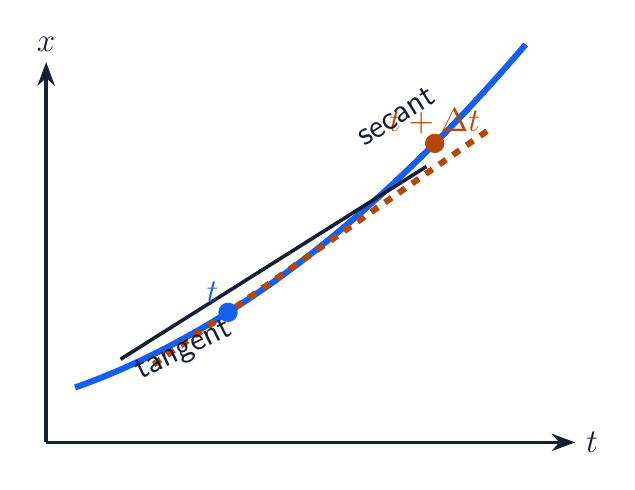
\begin{tikzpicture}[x=1.05cm,y=1.05cm]
  \draw[mech axis,-{Stealth[length=3mm,width=2.2mm]}] (0,0) -- (6.4,0) node[right] {\(t\)};
  \draw[mech axis,-{Stealth[length=3mm,width=2.2mm]}] (0,0) -- (0,4.6) node[above] {\(x\)};
  \draw[mech primary,domain=0.35:5.8,samples=80,smooth] plot (\x,{0.55+0.30*\x+0.075*\x*\x});
  \coordinate (P) at (2.2,{0.55+0.30*2.2+0.075*2.2*2.2});
  \coordinate (Q) at (4.7,{0.55+0.30*4.7+0.075*4.7*4.7});
  \draw[mech secondary] (1.3,{0.55+0.30*2.2+0.075*2.2*2.2-0.63}) -- (5.4,{0.55+0.30*2.2+0.075*2.2*2.2+2.24});
  \draw[mechInk,line width=1.3pt] (0.9,{0.55+0.30*2.2+0.075*2.2*2.2-0.567}) -- (4.6,{0.55+0.30*2.2+0.075*2.2*2.2+1.764});
  \fill[mechBlue] (P) circle (3.5pt) node[above left] {\(t\)};
  \fill[mechOrange] (Q) circle (3.5pt) node[above] {\(t+\Delta t\)};
  \node[rotate=32,above] at (4.35,3.75) {secant};
  \node[rotate=26,below] at (1.55,1.35) {tangent};
\end{tikzpicture}
\end{document}
